\chapter{Comparison of Methods}

This chapter compares the performance of various methods used in the UAV navigation system, focusing on accuracy, runtime, and robustness. The evaluation includes feature detectors, local feature matchers, rotational and translational estimators, and optimization techniques. Each method is tested across multiple datasets to assess generalization and suitability for real-world UAV applications.

\section{Testing Setup}

This section outlines the framework used to evaluate the performance of the proposed UAV navigation methods. The evaluation focuses on three primary metrics: accuracy, runtime, and robustness. These metrics are critical to ensure that the navigation system can reliably operate under diverse and challenging conditions, reflecting real-world scenarios where the UAV may encounter varying environmental factors.

Note that the testing setup is largely reused, and not reexplained, in the results chapter. 


\subsection{Critical Testing Pipeline Understanding}
The aim of these tests were to compare different methods and not to evaluate the system as a whole. These tests were not tested under optimal runtime or accuracy settings; however, other stages and parameters are held constant when testing between methods in a given stage. Further, sufficiently optimal non-testing parameters and methods were chosen such that the methods are tested under their intended optimal conditions. The results are not indicative of the overall performance of the system, and no comments thereon are made in this chapter. Specifically, no objective conclusions may be made about the overall performance in this chapter. 

Secondly, to ensure maximal usage of the dataset, the same images are used carefully in both the GPS and no GPS stages to ensure no bias. In the GPS Available phase, all 15 images are streamed and added, storing their features and telemetry. Further, the first 5 images are used to infer the fixed pixel to metre factor, related to the camera focal length and UAV altitude. Thereafter, in the no GPS phase, the last 14 images have their location and heading estimate. Naturally, each image recomputes its features, and does not infer its location based on its own image from the GPS pipeline, to ensure a fair test. 

\subsection{Datasets}

Five distinct datasets were selected to rigorously evaluate the methods' generalization and performance across diverse environments. These datasets were captured using Google Earth and involved both translational and rotational movements, simulating typical UAV navigation tasks. Although the primary transformations were translation and rotation, perspective distortions and other subtle deformations were present due to the uneven terrain. Multiple methods with varying degrees of freedom were tested to implicitly estimate which of these transforms were significantly present. Each of the properties and choices were done to ensure the task was challenging but not impossible.

\textbf{General Properties of the Datasets:}
\begin{itemize}
    \item \textbf{Altitude:} Ranging from 5.5 to 6.5 km, constant within each dataset. This is standard for UAV navigation applications and ensures the ground is sufficiently planar.
    \item \textbf{Resolution:} 1920x972 pixels per image. This is the standard resolution in most applications. Stress tests were performed at lower resolutions.
    \item \textbf{Radial Movement Between Frames:} Varies between 100 and 700 pixels depending on the image and the best match found, as is the case in reality. This variability does not impact inter-method comparisons. Metres are used for physical clarity, where, despite differences in scaling, a lower metre error directly indicates a lower percentage error between methods.
    \item \textbf{Number of Images per Dataset:} 15 images per dataset. This balances testing time and is sufficient to evaluate the methods' performance. 
\end{itemize}

The datasets used for testing were as follows:

\begin{itemize}
    \item \textbf{CITY1 and CITY2 (Cape Town):}  
    Both datasets were captured in Cape Town. \textbf{CITY1} includes both rotational and translational changes between frames, while \textbf{CITY2} is the only dataset that only focuses on translational movements. This distinction allows for isolated testing of performance under rotational stress.
    
    \item \textbf{ROCKY:}  
    This dataset, taken in the semi-arid Karoo region, involved rugged terrain with sparse vegetation. They involve translations and rotations. 
    
    \item \textbf{DESERT and AMAZON:}  
    The desert dataset was captured in the Sahara Desert, while the Amazon dataset was captured in the Amazon Rainforest. These datasets are characterized by sparse, repetitive patterns, making it challenging even for human observers to distinguish differences between frames. They present significant difficulty for feature extraction and matching. They both involve translations and rotations.
\end{itemize}

Examples of the datasets are shown below:

\begin{figure}[H]
    \centering
    \begin{minipage}{0.45\textwidth}
        \centering
        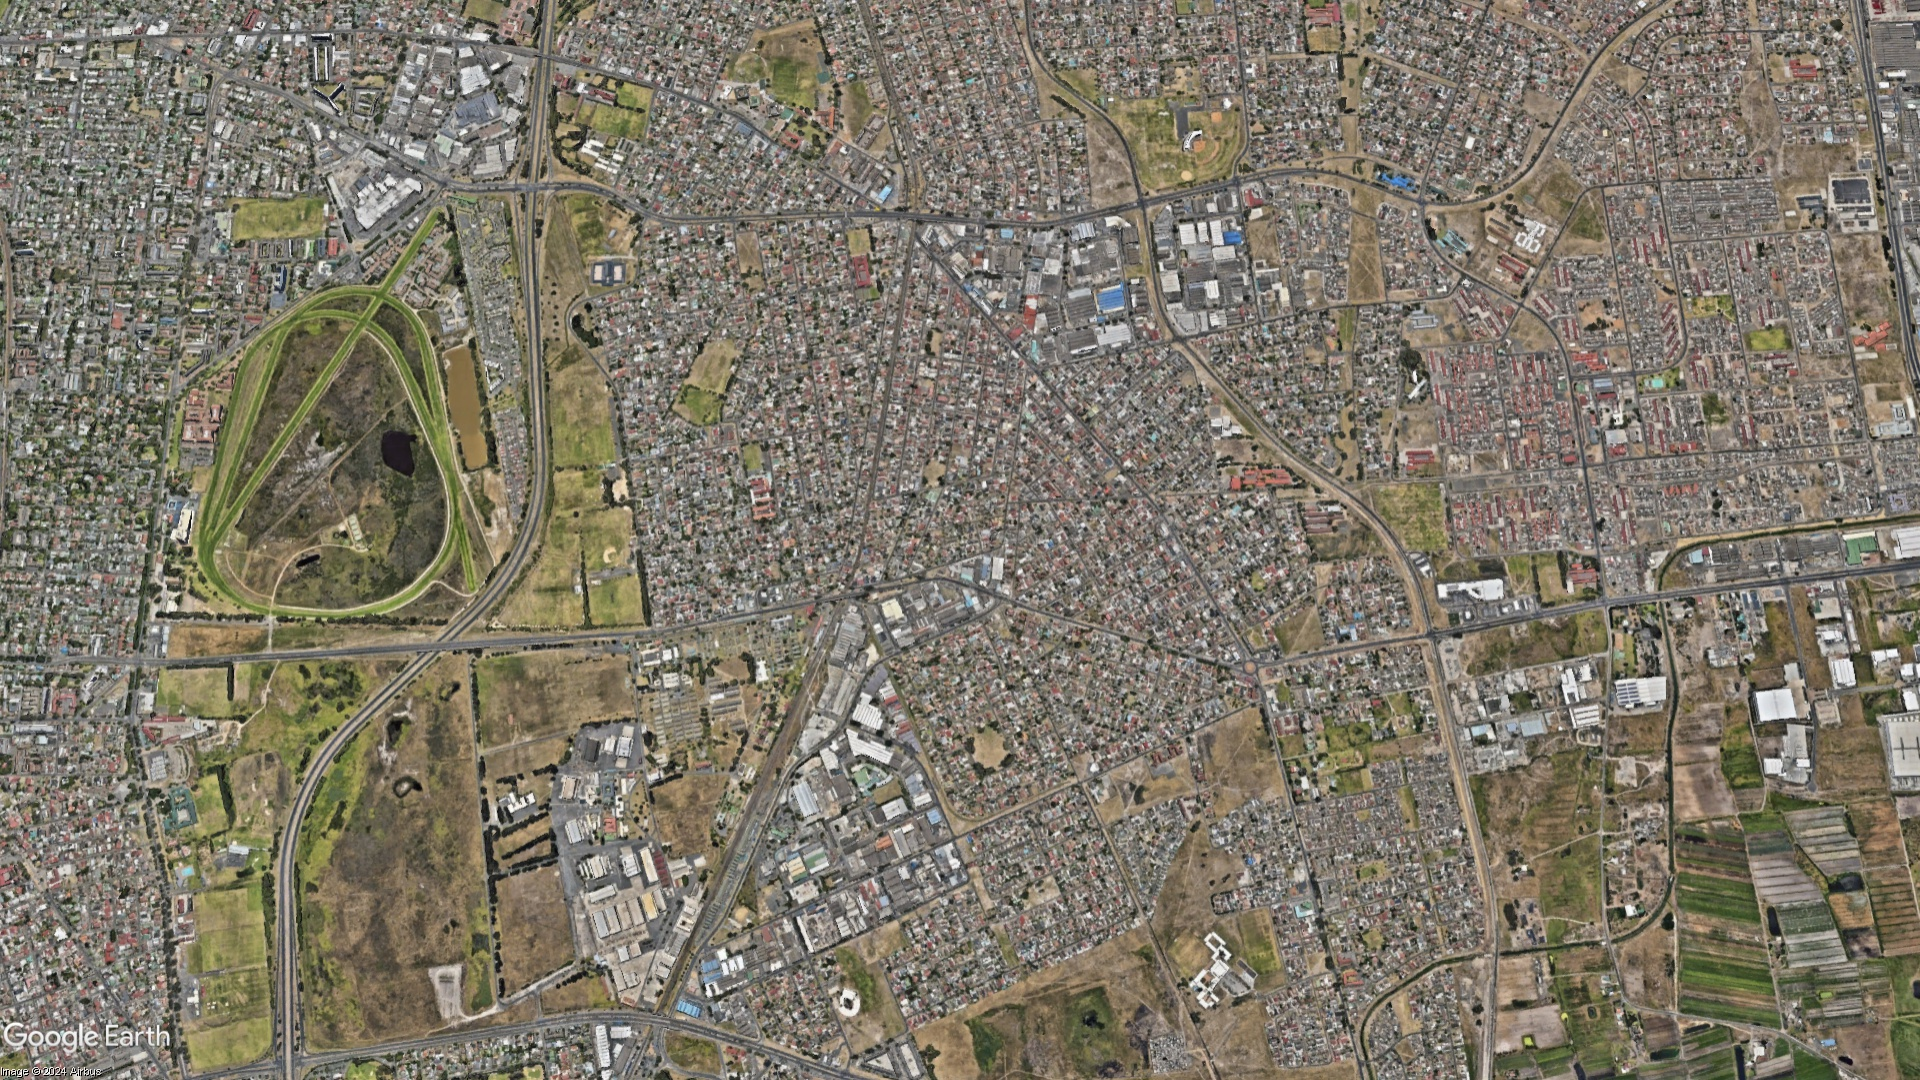
\includegraphics[width=\textwidth]{./Chapter 4/DEMODATASETS/CITY1.jpg}
        \caption{Examples of the CITY1 and CITY2 Datasets.}
        \label{fig:CITY12}
    \end{minipage}\hfill
    \begin{minipage}{0.45\textwidth}
        \centering
        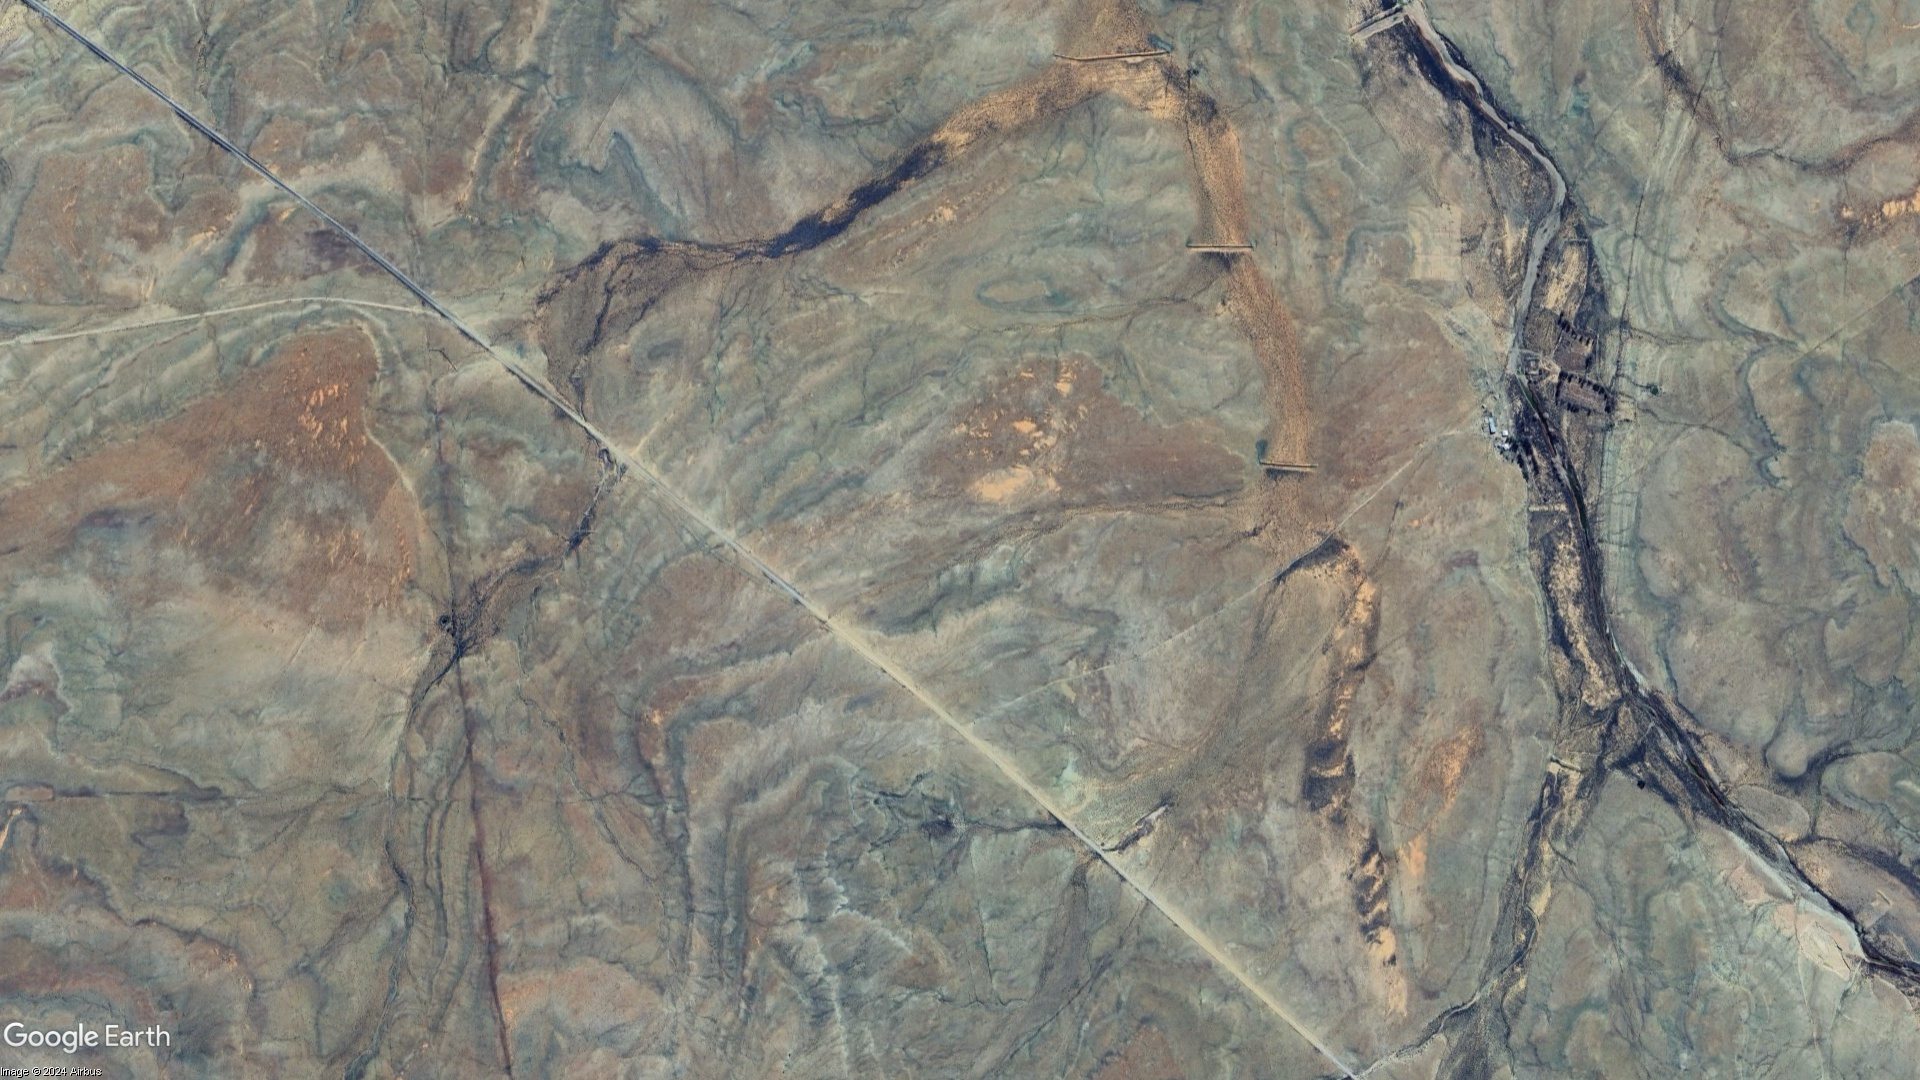
\includegraphics[width=\textwidth]{./Chapter 4/DEMODATASETS/ROCKY.jpg}
        \caption{Example of the ROCKY Dataset.}
        \label{fig:ROCKY}
    \end{minipage}
    
    \vspace{0.5cm} % Add some vertical space between rows
    
    \begin{minipage}{0.45\textwidth}
        \centering
        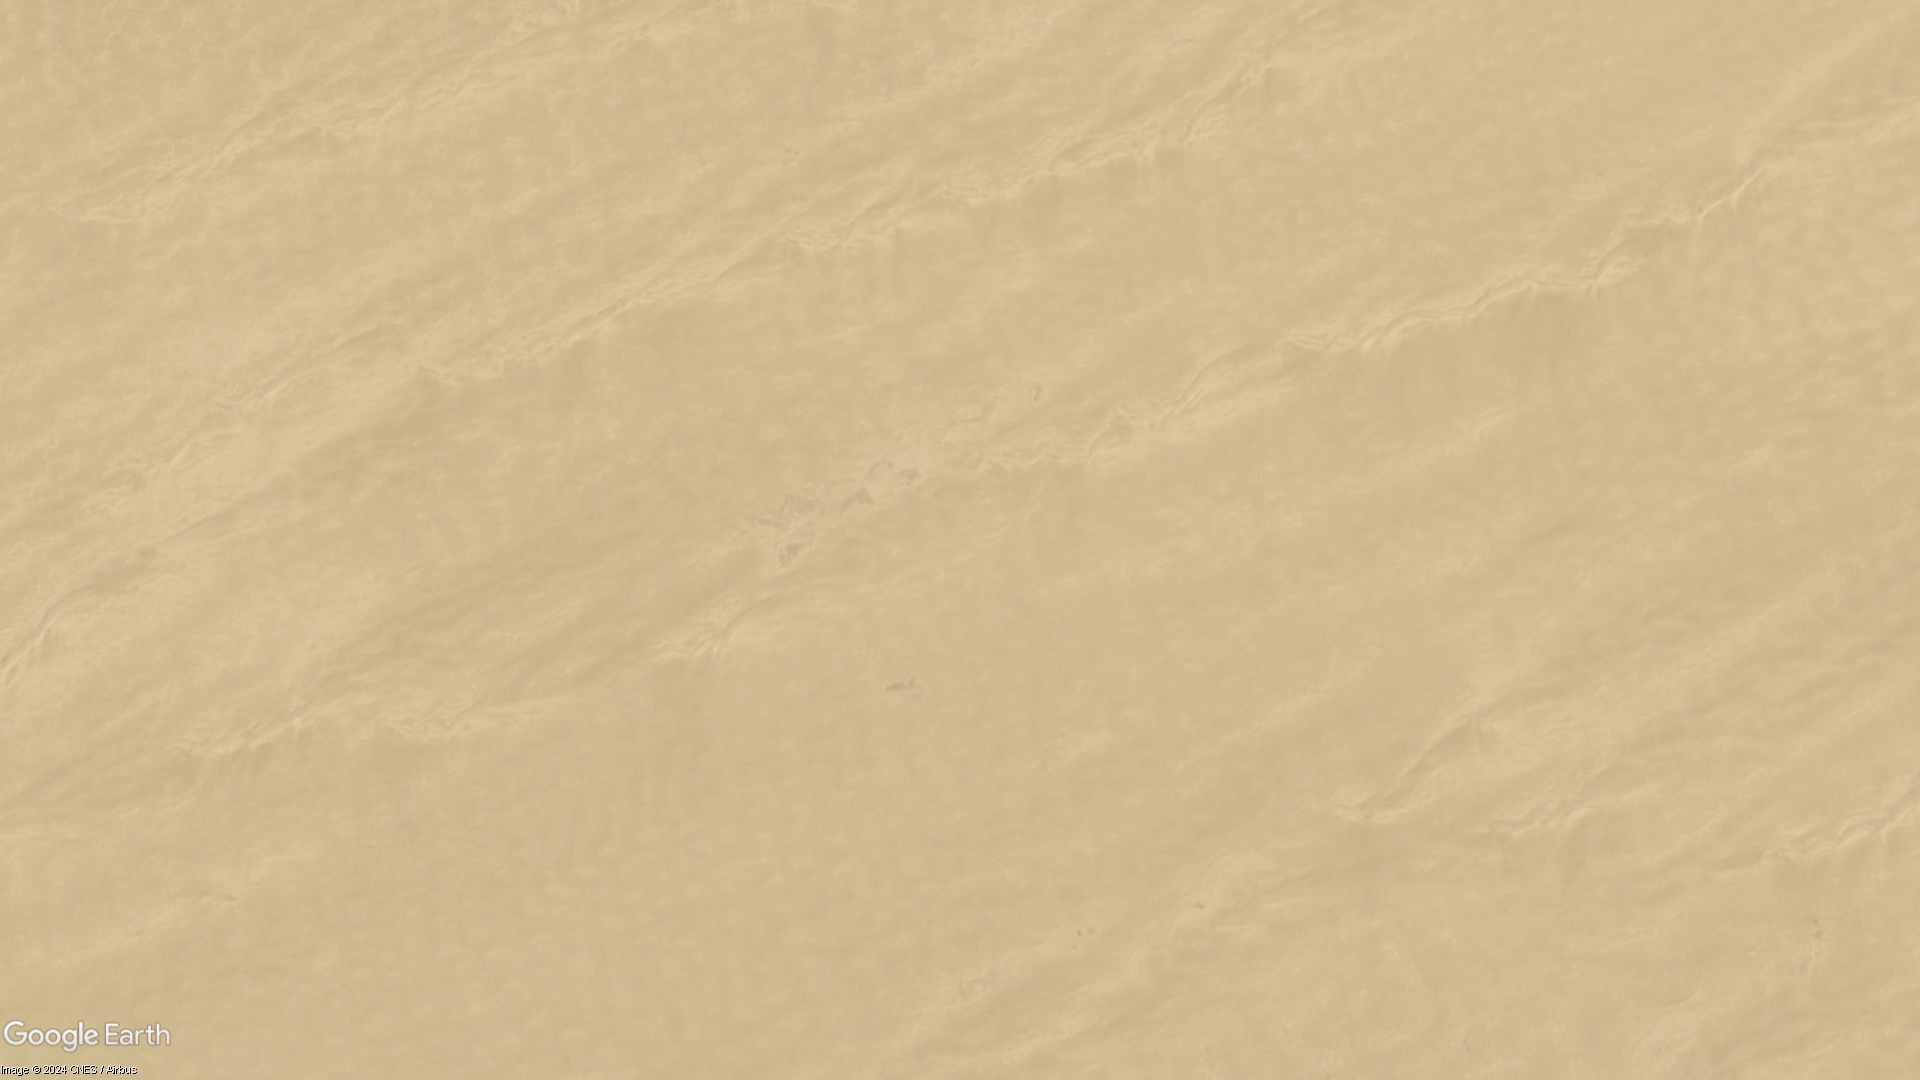
\includegraphics[width=\textwidth]{./Chapter 4/DEMODATASETS/DESERT1.jpg}
        \caption{Example of the DESERT Dataset.}
        \label{fig:DESERT}
    \end{minipage}\hfill
    \begin{minipage}{0.45\textwidth}
        \centering
        
\includegraphics[width=\textwidth]{./Chapter 4/DEMODATASETS/AMAZON.jpg}
        \caption{Example of the AMAZON Dataset.}
        \label{fig:AMAZON}
    \end{minipage}
    
    \caption{Overview of Datasets}
    \label{fig:Datasets}
\end{figure}



\subsection{Testing Structure}

Each method is subjected to rigorous testing based on the following criteria:

\begin{itemize}
    \item \textbf{Accuracy}: Evaluated using the radial Root Mean Square Error (RMSE) of GPS estimations, in metres. This metric is chosen, instead of percentage error, for a physical interpretation of the error, providing a clear indication of the method's accuracy in estimating the UAV's position. This does not compromise the inter-method comparisons, as the same metric is used across all methods. Further, this accuracy is only tested at the end of the pipeline, since any error or poor choice in prior stages will always propagate to the final GPS error; and often, the accuracy and impact of intermediate stages are not directly interpretable. This radial error is given as the mean of the radial errors for all images in the dataset. 
    
    \item \textbf{Runtime}: The runtime of the entire dataset is used as the method of comparison. This implies the runtime to compute all 15 images, for both the GPS and no GPS phases. As before, intermediary stages propagate this error, and the runtime per line is not necessarily indicative of better performance; Runtime per line is not tested. For instance, a method may quickly compute filtering, but if it does not filter much, later stages will be slower.
    slower.
    \item \textbf{Robustness}: This test specifically employs qualitative testing to evaluate the method's performance under variation in its parameters. That is, how hard is this method to tune, and how does it perform with crudely chosen parameters across datasets. This aims to evaluate the method's generalizability and robustness across diverse environments. A scoring system is developed to balance the nuances of parameter sensitivity evaluation by considering the range of parameters that can be chosen, and the performance of that range across datasets. Specifically, the scoring system, from 1-5, is as follows: 
        \begin{itemize}
            \item 5 indicates a wide range of parameters offer near perfect (defined as the performance of the most optimal parameter) performance across datasets,
            \item 4 indicates a large range of parameters offer good performance across datasets or a small range offers near perfect performance,
            \item 3 indicates a small range of parameters offer good performance across datasets,
            \item 2 indicates a small range of parameters offer significantly performance across datasets, and
            \item 1 indicates that no static threshold will work across datasets.
        \end{itemize}
    
\end{itemize}


    
This structured testing approach ensures that each component of the UAV navigation system is thoroughly evaluated, facilitating the selection of methods that deliver optimal performance across all critical metrics.





\section{Feature Detectors}

This section presents the evaluation results of three feature detectors: ORB, AKAZE, and SuperPoint with LightGlue. Feature detectors were applied to extracting a crude feature layer for rotational estimation, as well as a dense layer for rotational and translational estimation. Initially, all 3 transformations were tested independently for each detector, however, it was seen that the inter-method comparison conclusions were equivalent for each stage. Therefore, to maintain brevity, the detectors are applied to all stages and compared once, with the understanding of equivalent comparative independent responses to each stage.

\subsection{Accuracy and Runtime}

Figure ~\ref{fig:rmse_detectors} and Figure ~\ref{fig:runtime_detectors} present the radial error and runtime values for each feature detector across different datasets. AKAZE, utilizing dynamic keypoint targeting, demonstrated the highest accuracy across all datasets while maintaining reasonable runtime. SuperPoint recorded the highest radial errors, particularly in challenging datasets such as ROCKY and AMAZON, indicating its limited generalizability across diverse environments due to its training set. Meanwhile, ORB proved to be the most efficient detector, making it suitable for applications requiring fast processing. SuperPoint demonstrated the longest runtimes across all datasets, highlighting its limited applicability for time-sensitive applications unless optimized with GPU acceleration.

\begin{figure}[H]
    \centering
    \begin{minipage}{0.45\textwidth}
        \centering
        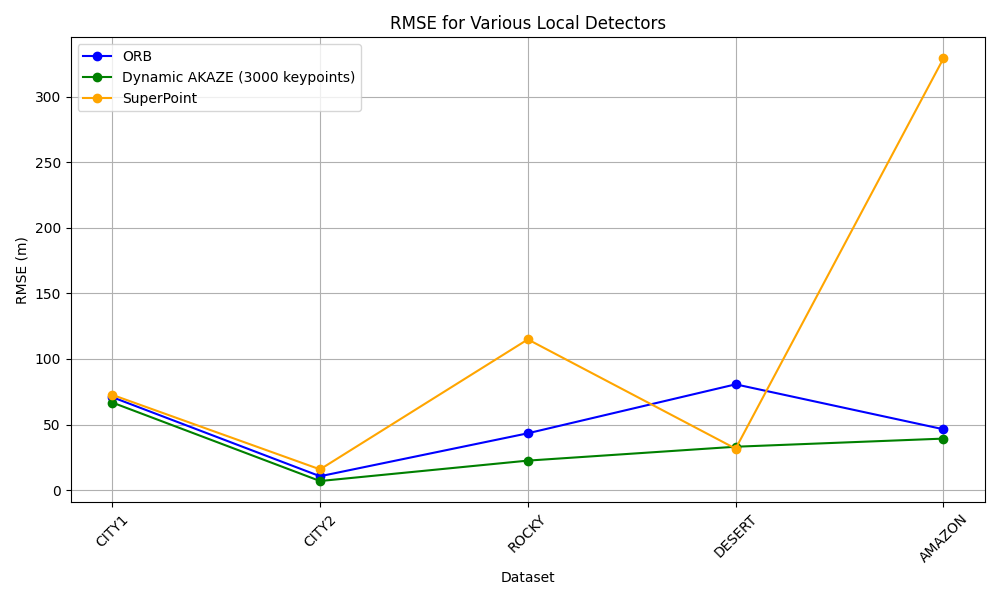
\includegraphics[width=\textwidth]{./Chapter 4/testresults/rmse_detectors.png}
        \caption{Radial Error for Various Local Detectors.}
        \label{fig:rmse_detectors}
    \end{minipage}\hfill
    \begin{minipage}{0.45\textwidth}
        \centering
        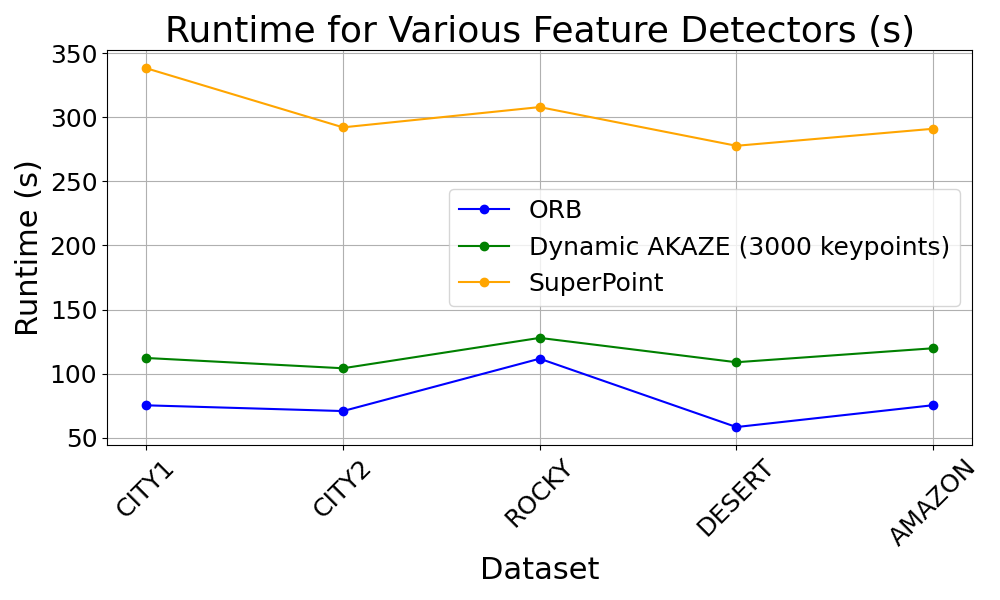
\includegraphics[width=\textwidth]{./Chapter 4/testresults/runtime_detectors.png}
        \caption{Runtime for Various Local Detectors.}
        \label{fig:runtime_detectors}
    \end{minipage}
    \caption{RMSE and Runtime Comparison for ORB, AKAZE, and SuperPoint Across Datasets.}
    \label{fig:rmse_runtime_detectors}
\end{figure}


\subsubsection{Robustness}

All the 3 methods were able to maintain their keypoint targets across environments; AKAZE is evaluated in terms of its dynamic keypoint targeting implementation. However, the quality of keypoints varied significantly across datasets, leading to variant performances, showing the downsides of static keypoint targeting. SuperPoint consistently achieved good performance across multiple keypoint targets, achieving it a robustness score of 5. AKAZE, with its dynamic targeting, was able to generalize well across datasets and only significantly dropped in performance when using below 1000 keypoints, achieving a robustness score of 4. ORB, while efficient, required precise tuning to achieve consistently good performance across datasets and was highly sensitive to the target parameter, achieving a robustness score of 3.

\subsection{Final Selection of Feature Detectors}

Based on the comprehensive evaluation, the following detectors were selected for the respective stages of the UAV navigation system:

\begin{itemize}
    \item \textbf{Crude Layer (Initial Detection)}: \textbf{ORB} was chosen for the crude, rotational estimation layer due to its balance of accuracy and efficiency. A range of 3000 - 8000 keypoints maintained reasonable accuracy and runtime, largely due to the invariance of the image similarity estimators to rotational inaccuracies. 3000 keypoints was chosen to prioritize speed and maintain FLANN runtime as per \ref{sec:FLANN_BF_Considerations}.
    
    \item \textbf{Dense Layer (Refined Detection)}: \textbf{Dynamic AKAZE} was selected for the dense layer due to its consistent performance and robustness and applied to both rotational and translational estimation stages. A range of 3000-5000 maintained consistent runtime and accuracy. 3000 keypoints was chosen to balance runtime, accuracy and maintain FLANN runtime as per \ref{sec:FLANN_BF_Considerations}.
\end{itemize}


\section{Local Feature Matchers}

This section evaluates two prominent local matchers, BFMatcher and FLANN, within the context of a UAV navigation system. Note that LightGLue was implicitly tested in the feature detectors section with SuperPoint, as explained in the prior two sections. 

\subsection{Accuracy and Runtime Evaluation}

Figure \ref{fig:rmse_flann_bf} presents the radial error in GPS values for BFMatcher and FLANN across different datasets. The results indicate that while BFMatcher achieves slightly better accuracy in certain cases, FLANN remains highly competitive with only marginally higher RMSE values.

Figure \ref{fig:runtime_flann_bf} shows the runtime comparison for BFMatcher and FLANN across different datasets. FLANN consistently outperforms BFMatcher in terms of speed, with significantly lower execution times across all datasets.Specifically, in the CITY datasets, where the number of keypoints found were significantly higher, despite keypoint targeting, BFMatcher's runtime was significantly higher than FLANN's. This is attributed to FLANN's approximate matching, which scales better with the number of keypoints.

\begin{figure}[H]
    \centering
    \begin{minipage}{0.45\textwidth}
        \centering
        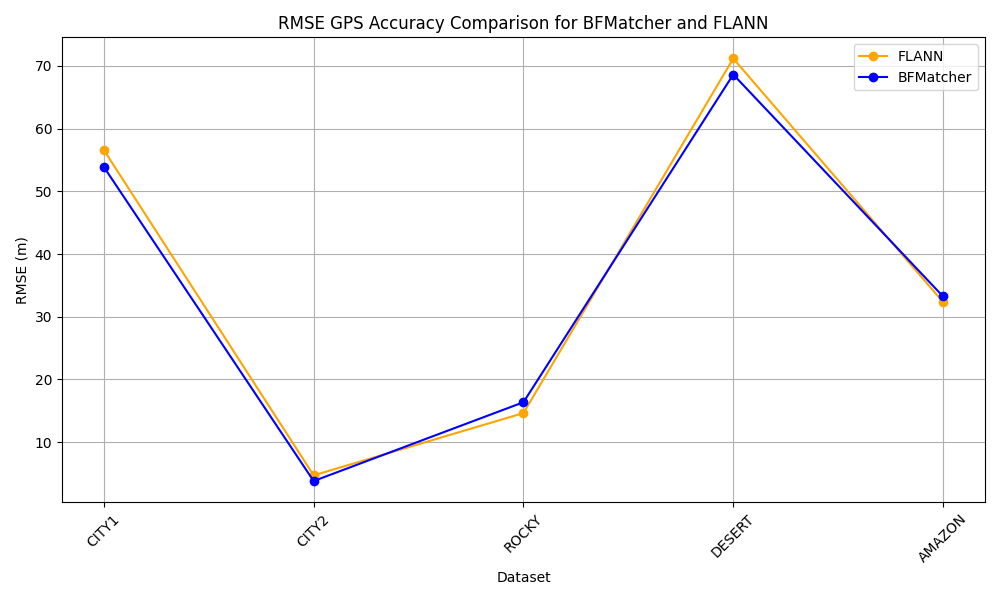
\includegraphics[width=\textwidth]{./Chapter 4/testresults/rmse_flann_bf.png}
        \caption{Radial Error for BFMatcher and FLANN.}
        \label{fig:rmse_flann_bf}
    \end{minipage}\hfill
    \begin{minipage}{0.45\textwidth}
        \centering
        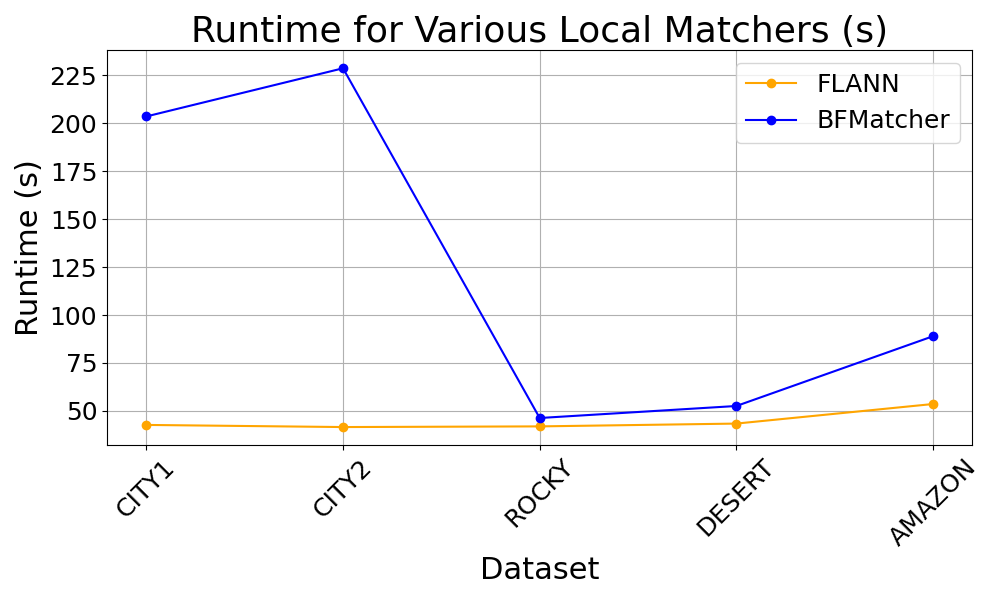
\includegraphics[width=\textwidth]{./Chapter 4/testresults/runtime_flann_bf.png}
        \caption{Runtime Comparison for BFMatcher and FLANN.}
        \label{fig:runtime_flann_bf}
    \end{minipage}
\end{figure}



\subsection{Robustness Testing}
BFMatcher did not have any tunable parameters. FLANN did, however, it showed limited variation in accuracy across the entire spectrum of parameters. As such, both methods achieve a robustness score of 5.

\subsection{Considerations}
\label{sec:FLANN_BF_Considerations}
This section details the scenarios in which each method should be employed. Figure ~\ref{fig:FLANN BF Matcher Keypoint Convergence} depicts the convergence in RMSE GPS error between FLANN and BFMatcher as the number of keypoints increases. Positive values indicate that BFMatcher outperforms FLANN, while negative values suggest FLANN performs better. The plot demonstrates the convergence in accuracy of both matchers as the number of keypoints increases, with FLANN generally maintaining slightly higher RMSE values than BFMatcher. Note that outliers are present, indicating instances where FLANN achieves better accuracy than BFMatcher. This is attributed to FLANN's approximate matching, paired with a static Lowe's ratio threshold, which may preserve valid matches that BFMatcher might discard due to finding a better second match. Notably, if FLANN is to be employed, at least 3000 keypoints should be targeted to ensure consistent performance across datasets. If significantly below this, BF matcher should be considered. 

\begin{figure}[H]
    \centering
    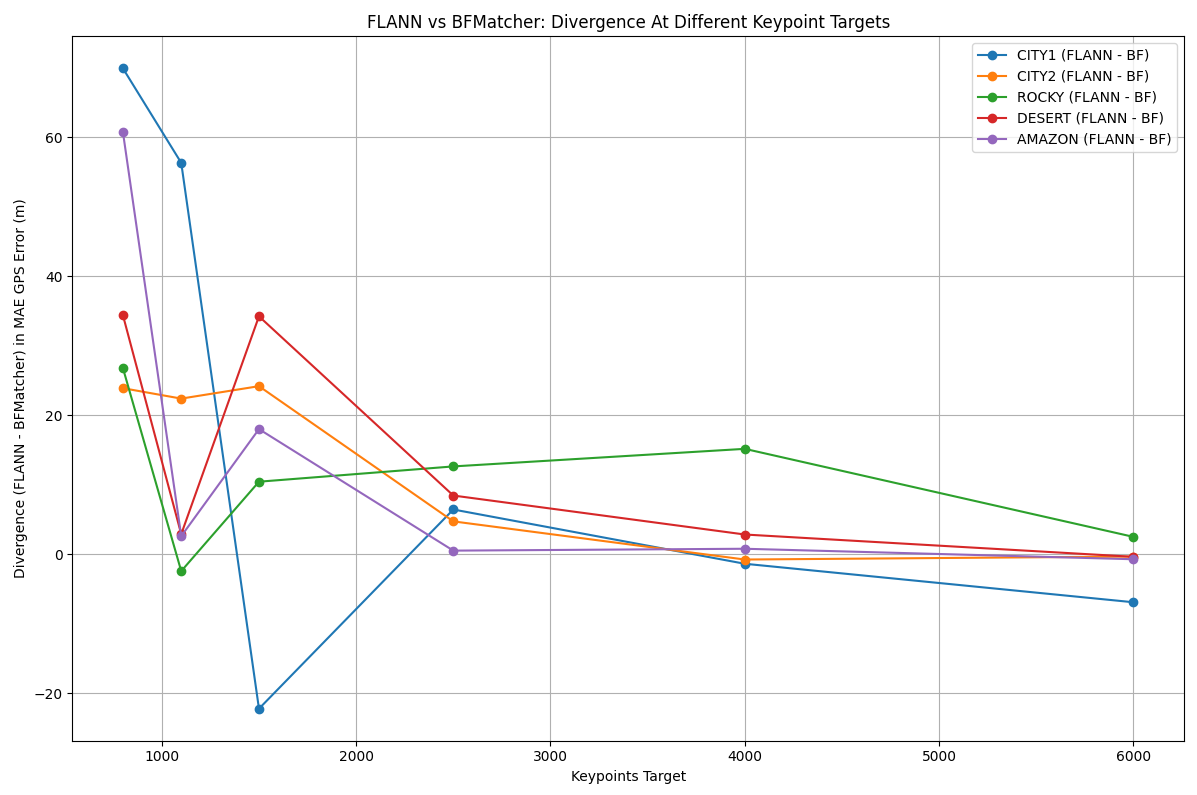
\includegraphics[width=0.8\textwidth]{./Graphs/Divergence_BF_FLANN_KPS.png}
    \caption{Convergence in RMSE GPS Error Between FLANN and BFMatcher Across Keypoint Targets.}
    \label{fig:FLANN BF Matcher Keypoint Convergence} 
\end{figure}


\subsection{Final Selection of Local Feature Matcher}

Based on the comprehensive evaluation of accuracy, runtime, and robustness, FLANN emerges as the optimal choice for the UAV navigation system. FLANN offers significantly faster runtimes and better scalability while maintaining comparable accuracy to BFMatcher. However, at least 3000 keypoints should be targeted to ensure consistent performance across datasets.


\section{Planar Transform Estimators}

This section evaluates the performance of four planar transformation estimation methods: Partial Affine 2D (Rigid Transform plus minor Scaling), Affine 2D, Homography, and Rigid Transform Via SVD. As noted in section \ref{sec:testing_shortlist}, both rotational and translational stages are combined into a single transform evaluation due to conclusion equivalency. For these tests, RANSAC was used on all methods, except the Rigid Transform Via SVD which does not have the method built-in, to filter outliers.

\subsection{Accuracy and Runtime Evaluation}

Figure \ref{fig:rmse_runtime_comparison_rotestim} summarizes the RMSE and runtime values across datasets for each rotational estimator method. From the results, it is clear that each method exhibits strengths in different datasets. However, the Rigid SVD method and Partial Affine 2D consistently emerge as the most accurate methods. This implies that the Rigid SVD transform provides the most stable and accurate estimate of the rotational and translational components of the UAV's movement. The Rigid SVD method slightly outperforms Partial Affine 2D in most datasets, attributed to its strict rigid transformation alignment with dataset characteristics.

The runtime results, shown in \ref{fig:rmse_runtime_comparison_rotestim}, are influenced by the degrees of freedom in each method, with rigid-based transforms demonstrating the best performance across datasets. SVD proves the fastest due to its lack of iterative optimization.


\begin{figure}[H]
    \centering
    \begin{minipage}{0.45\textwidth}
        \centering
        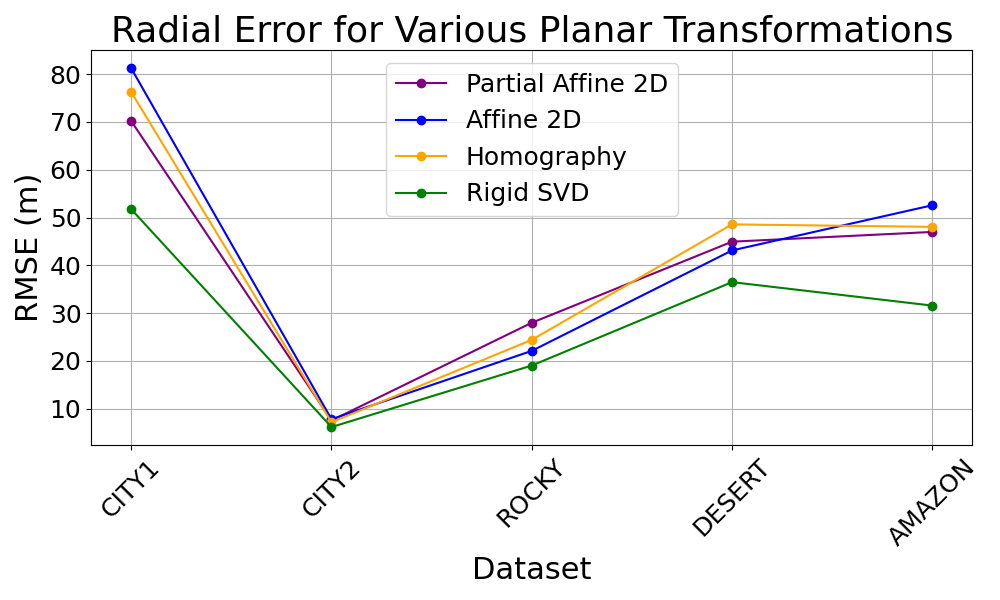
\includegraphics[width=\textwidth]{./Chapter 4/testresults/rmse_planar_estimators.png}
        \caption{RMSE Comparison Across Datasets for Planar Transform Estimators.}
    \end{minipage}\hfill
    \begin{minipage}{0.45\textwidth}
        \centering
        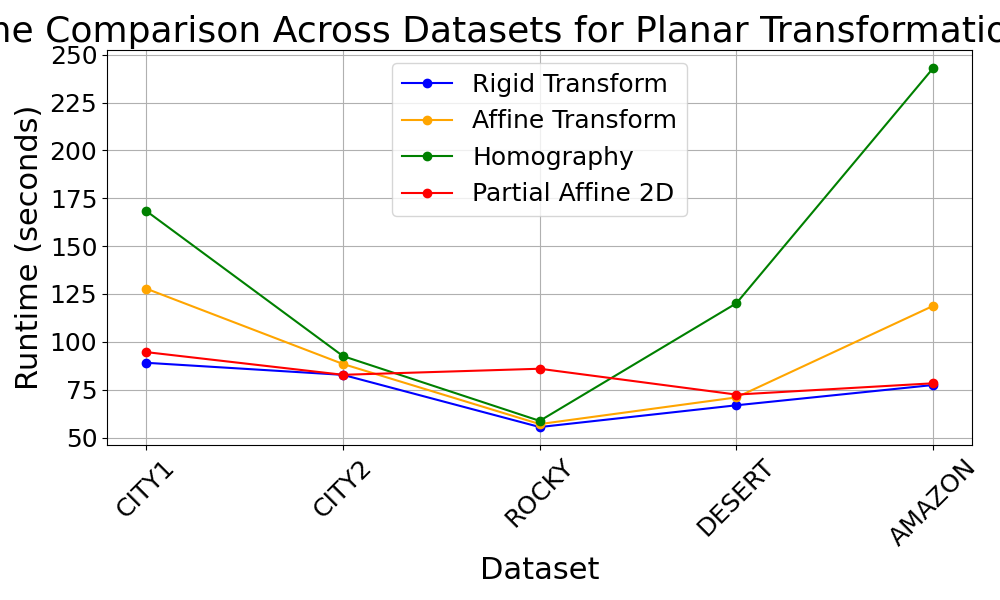
\includegraphics[width=\textwidth]{./Chapter 4/testresults/runtime_planar_estimators.png}
        \caption{Runtime Comparison Across Datasets for Planar Transform Estimators.}
    \end{minipage}
    \caption{RMSE and Runtime Comparison Across Datasets for Planar Transform Estimators.}
    \label{fig:rmse_runtime_comparison_rotestim}
\end{figure}
   
    

\subsection{Robustness Testing}

The openCV methods (partial Affine 2D, Affine 2D, homography) utilize RANSAC, or less often, LMEDS or other outlier rejection methods for robust outlier rejection. These thresholds subtended large differences in accuracy when varied, and required threshold testing from very low to very high thresholds to find the optimal threshold. For more complex, 3-Dimensional, transformations this threshold may be more useful, but it was found to not beat the accuracy of the Rigid SVD method under any threshold in the given application. Thus, OpenCV methods achieve a score of 3 for robustness, while the Rigid SVD method achieves a score of 5 due to its lack of tunable parameters. 

\subsection{Final Selection of Rotational Estimator}

Based on the comprehensive evaluation of accuracy, runtime, and robustness, the rigid transform by SVD emerged as the most suitable estimator for the UAV navigation system. It demonstrated the lowest combined radial RMSE in GPS across all datasets, and the fastest runtime, largely due to its application-aligned degrees of freedom. Further, it required no parameter tuning, making it highly suitable for real-time UAV applications.





\section{Image Similarity Estimators}

Accurate image similarity estimation, or global matching, is essential for UAV navigation systems to choose reasonable images to compare to. They should ensure accuracy and efficiency while maintaining robustness against small rotational offsets. The proximity radius for initial search space reduction was crudely set to 5, but this is not tested as it is a design choice dependent on external factors such as the UAV's speed and the image capture rate. This section specifically evaluates the global matching techniques which are used to estimate the similarity between images to infer the closest match for subsequent heading and position estimation. 


\subsection{Accuracy and Runtime Evaluation}

For clarity, the best match found is implicitly realized in the GPS estimation error because more similar matches will have more accurate correspondences and subsequently subtend higher accuracy matches. 

Figure ~\ref{fig:rmse_global_matching} summarizes the RMSE values (in meters) for the Local Retrofit, Cross Correlation, Histogram, and SSIM methods. The results indicate that the Histogram and Cross-Correlation technique perform near equivalently, with SSIM marginally behind. The Local Retrofit method recorded the highest RMSE values, especially in the DESERT dataset, since its requirement for crude detection and matching to maintain runtime meant it could not find sufficient good matches on the sparsest of datasets; It was excluded from further analysis.

Figure ~\ref{fig:runtime_global_matching} compares the computational efficiency of each global matching technique across the five datasets. The Histogram technique demonstrated the most consistent runtimes, followed closely by Cross Correlation. SSIM exhibited the longest runtimes of the remaining methods due to its more complex structural similarity calculations. 


\begin{figure}[H]
    \centering
    \begin{minipage}{0.45\textwidth}
        \centering
        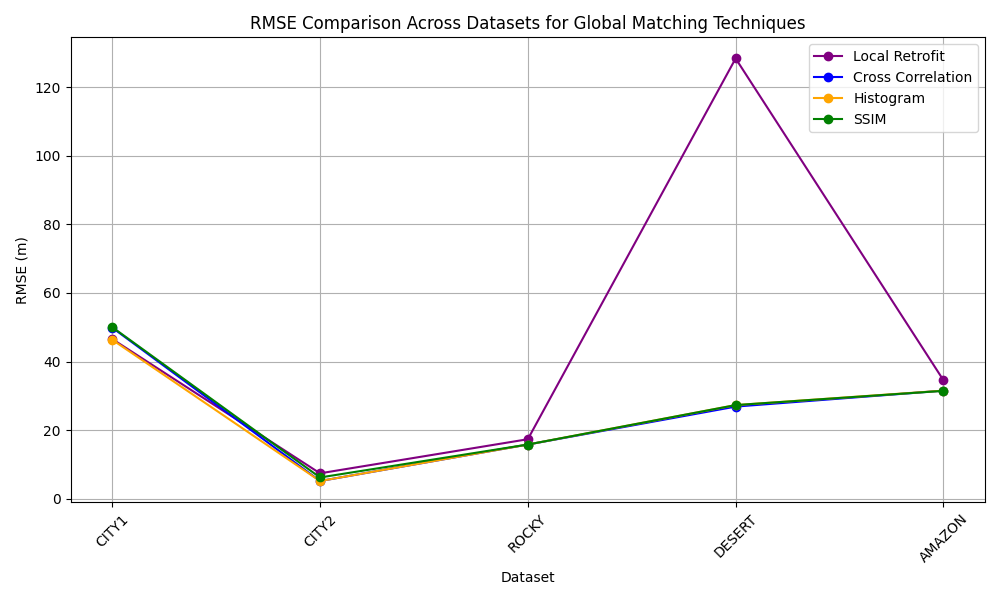
\includegraphics[width=\textwidth]{./Chapter 4/testresults/rmse_global_matching.png}
        \caption{RMSE Comparison Across Datasets for Global Matching Techniques.}
        \label{fig:rmse_global_matching}
    \end{minipage}\hfill
    \begin{minipage}{0.45\textwidth}
        \centering
        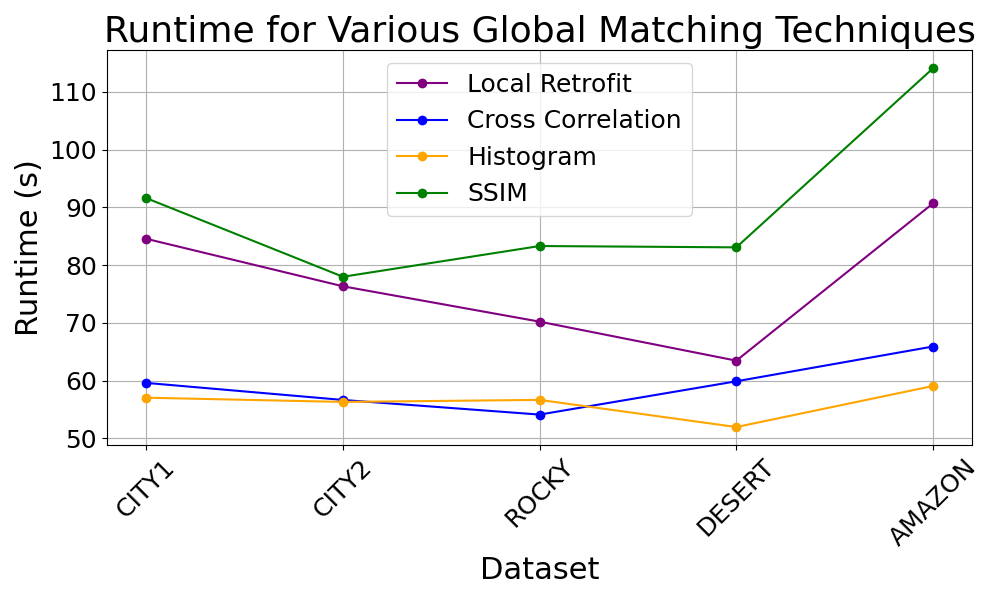
\includegraphics[width=\textwidth]{./Chapter 4/testresults/runtime_global_matching.png}
        \caption{Runtime Comparison Across Datasets for Global Matching Techniques.}
        \label{fig:runtime_global_matching}
    \end{minipage}
\end{figure}

\subsection{Robustness Testing}
The global matching methods did not have any tunable parameters, achieving them a robustness score of 5. However, the local retrofit model had various parameters that could be tuned, including detector type, detector threshold, grid size, match threshold. Further, the runtime and accuracy were extremely difficult to balance, requiring extremely precise tuning to achieve usable performance. As such, the local retrofit model achieved a robustness score of 2. 


\subsection{Considerations for Alignment Prior to GLobal Matching}

This sections details the considerations when choosing the precision of the rotational alignment techniques employed to align the image pairs for unbiased similarity comparisons  between the images. This test subjects the estimated internal alignment to an additional skew and notes their response in best match choice, realized through radial error. This was first tested under a 5-degree skew, where no changes occur. Figure ~\ref{fig:percentage_change_comparison_methods} shows the percentage change in GPS error from the prior estimate, with no skew, with a 10-degree skew. Cross-correlation maintains the most similar accuracy, closely followed by histogram and then SSIM. All methods are highly robust to rotational misalignments up to 5 degrees, however, should not exceed this. As such, when employing a rotational alignment technique prior to global matching, a 5-degree skew is tolerable and the choice of detector and matcher may be guided by efficiency rather than accuracy.


\begin{figure}[H]
    \centering
    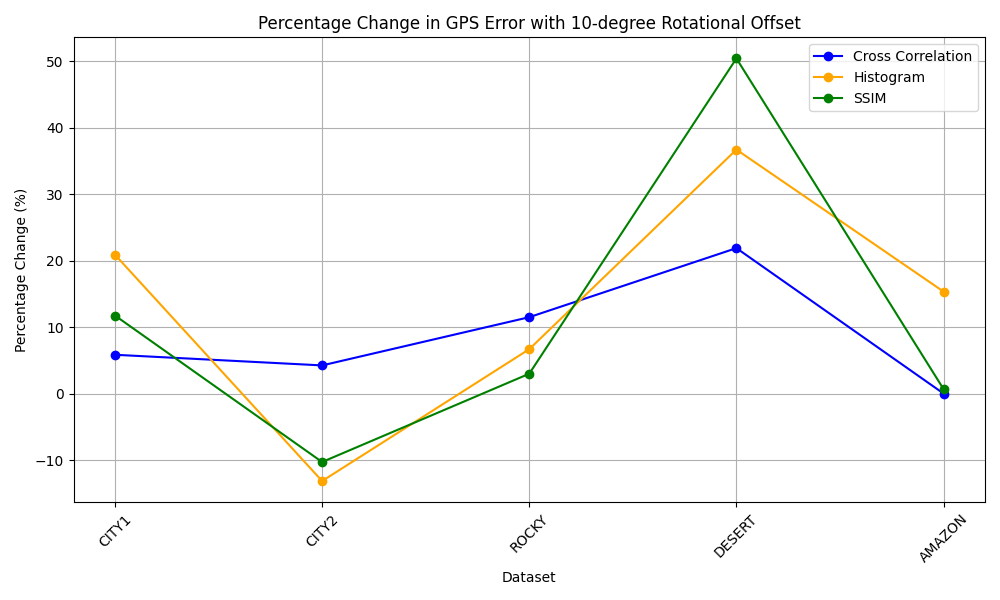
\includegraphics[width=\textwidth]{./Chapter 4/testresults/percentage_change_comparison_methods.png}
    \caption{Percentage Change in GPS Error with 10-degree Rotational Offset}
    \label{fig:percentage_change_comparison_methods}
\end{figure}





\subsection{Final Selection of Global Matching Technique}

Based on the comprehensive evaluation of accuracy, runtime, and robustness, the \textbf{Histogram} technique is identified and chosen as the most suitable global matching method for the system. Histogram consistently provided superior performance in terms of both RMSE and runtime, whilst maintaining sufficient robustness to rotational error. 




\section{Optimization Techniques}
Various methods were employed to improve the performance of the UAV navigation system. The optimization techniques focus on filtering matches between images to balance noise and stability in the point sets. 


This section outlines the selected optimization 

\subsection{Planar Transform Outlier Rejection Methods}

Two outlier rejection methods, LMEDS (Least Median of Squares) and RANSAC (Random Sample Consensus), were evaluated for match filtration. Both methods performed near equivalently, with LMEDS displaying a slightly lower radial error. LMEDS was also significantly faster than RANSAC, making it the preferred choice for planar transform outlier rejection. The results are summarized in Figure \ref{fig:rmse_comparisonlmeds} and Figure \ref{fig:runtime_comparisonlmeds}. Both thresholds require precise tuning, with LMEDS requiring slightly less tuning. Both methods achieved a robustness score of 3, as they required precise tuning to achieve optimal performance across datasets.

\begin{figure}[H]
    \centering
    \begin{minipage}{0.45\textwidth}
        \centering
        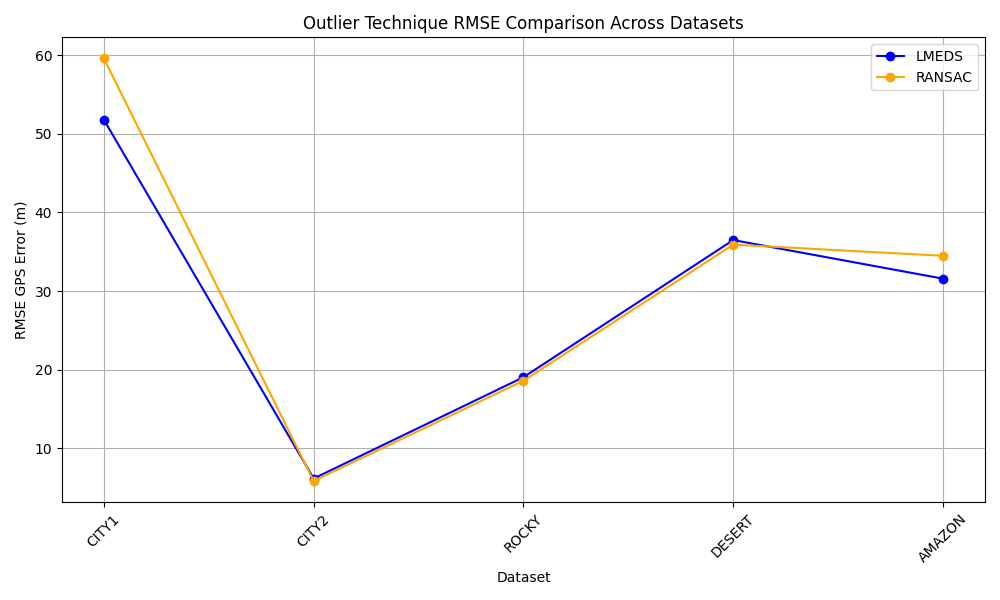
\includegraphics[width=\textwidth]{./Chapter 4/testresults/ransaclmedsrmse.png}
        \caption{Radial GPS RMSE Comparison Across Datasets for LMEDS and RANSAC}
        \label{fig:rmse_comparisonlmeds}
    \end{minipage}\hfill
    \begin{minipage}{0.45\textwidth}
        \centering
        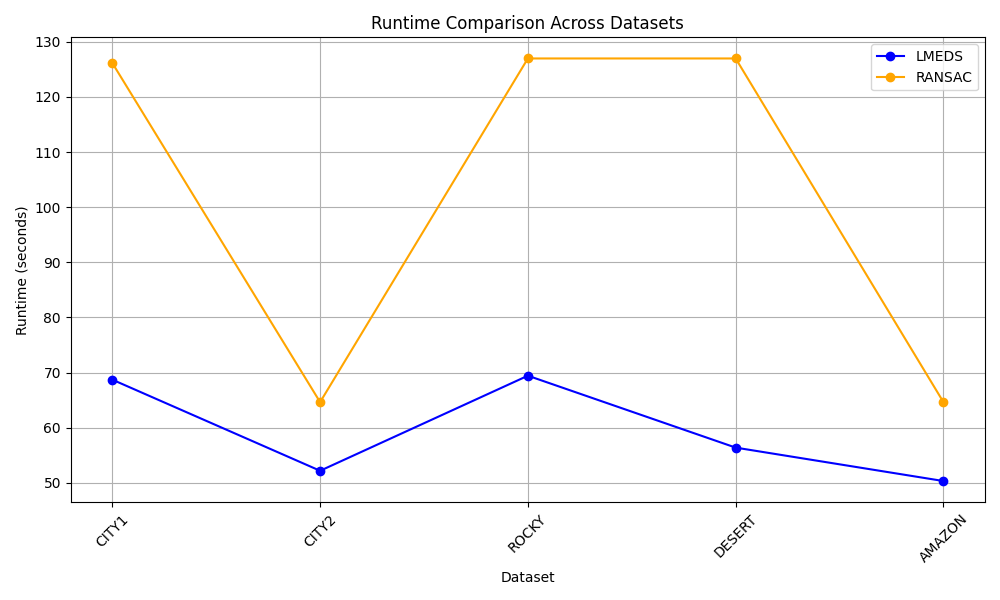
\includegraphics[width=\textwidth]{./Chapter 4/testresults/ransaclmedsruntime.png}
        \caption{Runtime Comparison Across Datasets for LMEDS and RANSAC}
        \label{fig:runtime_comparisonlmeds}
    \end{minipage}
\end{figure}



\subsection{Lowe's Ratio Test}

Lowe's ratio test was employed to filter keypoint matches by comparing the distance of the best match to the second-best match. A static threshold proved inadequate for generalizing across diverse datasets, leading to inconsistent accuracy. To enhance robustness, a dynamic thresholding approach was implemented. This required setting an initial threshold, and incrementing it, thereby increasing leniency until a certain number of matches, or percentage of the keypoints were found.  

The accuracy significantly changed depending on these parameters, achieving it a robustness score of 3. However, its impact on accuracy is undoubtedly essential, and the dynamic thresholding makes it significantly more applicable. 

The initial threshold was set to 0.7, and the increment was set to 0.05. The threshold was incremented until 75\% of the keypoints were matched, or until the 500 good matches were found. It was tested that setting the initial threshold and increment too far below this, such as 0.5 and 0.025 respectively, led to a increases in runtime. Setting the initial threshold above 0.8, or the increment above 0.1 led to inclusion of too many noisy matches. If the exit conditions were too low or high, the same effect was observed. The chosen thresholds are within an acceptable range without being perfectly optimal.


\subsection{{N-Match or Absolute Thresholding}}
These approaches leveraged fixed number or descriptor distance thresholds to filter matches. However, without relativity to the density and quality of keypoints, empirical tests revealed that these methods added instability to the system. They either had no meaningful effect or removed too many matches, leading to loss of accuracy. The thresholds were deemed too sensitive for generalized applications. 



\section{Summary}
The following methods were selected based on the comprehensive evaluation of accuracy, runtime, and robustness across diverse datasets:

\begin{itemize}
    \item \textbf{Feature Detectors:} ORB for the crude similarity alignment layer and Dynamic AKAZE for the dense transformation estimation layer.
    \item \textbf{Local Feature Matcher:} FLANN for its superior runtime and scalability.
    \item \textbf{Transformational Estimator:} Rigid Transform SVD for its high accuracy, fast runtime, and robustness.
    \item \textbf{Image Similarity Estimator:} Histogram for its superior accuracy and runtime.
    \item \textbf{Optimization Techniques:} Dynamic Lowe's filtering for enhanced match quality and consistency. LMEDS was not included due to prior choices of methods not requiring it.
\end{itemize}